\pagebreak
\section{Discussion}
\label{sec:discussion}

\subsection{Prototype Hardware}
% Add drawings / design philosophy 
The robot is designed with the Open Continuum Robotics project in mind. It uses easily accessible, off-the-shelf components, and 3D printed parts so that other groups can reconstruct the same robot. A full breakdown of the robot's physical design can be found in Appendix \ref{app:robot_drawings}. 

\subsubsection{Physical Description of Prototype}
\label{sec:physical_description}
% Arms
\paragraph{The arms} are each \SI{80}{cm} long and consist of a \SI{0.0200}{"} thick, \SI{0.75}{"} wide beam made from 1095 spring steel, with 19 evenly spaced 3D printed tendon spacers. The spacers hold one tendon on each side of the beam \SI{11}{mm} away from the steel beam. The 1095 spring steel beam is used as the central beam as it provides rigidity in the direction of motion off the robot's planar surface, while remaining flexible along the plane. The high elasticity of the material allows the system to undergo large curvatures without permanently deforming the beam. The tendons used are \SI{30}{lbs} braided fishing line (Super8Slick V2, Power Pro, CA, USA). Each tendon has four \SI{0.75}{"} nuts on it that act to maintain tension during operational periods where it is being extended. 

\begin{figure}[h]
    \centering
    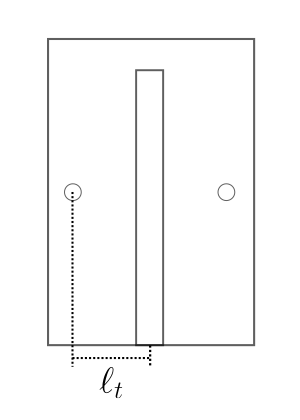
\includegraphics[width=0.3\textwidth]{images/beam_cross_section.png}
    \caption{Cross section of the beam spacers. $\ell_t = \SI{11}{mm}$}
    \label{fig:beam_cross_section}
\end{figure}

\begin{figure}[h]
    \centering
    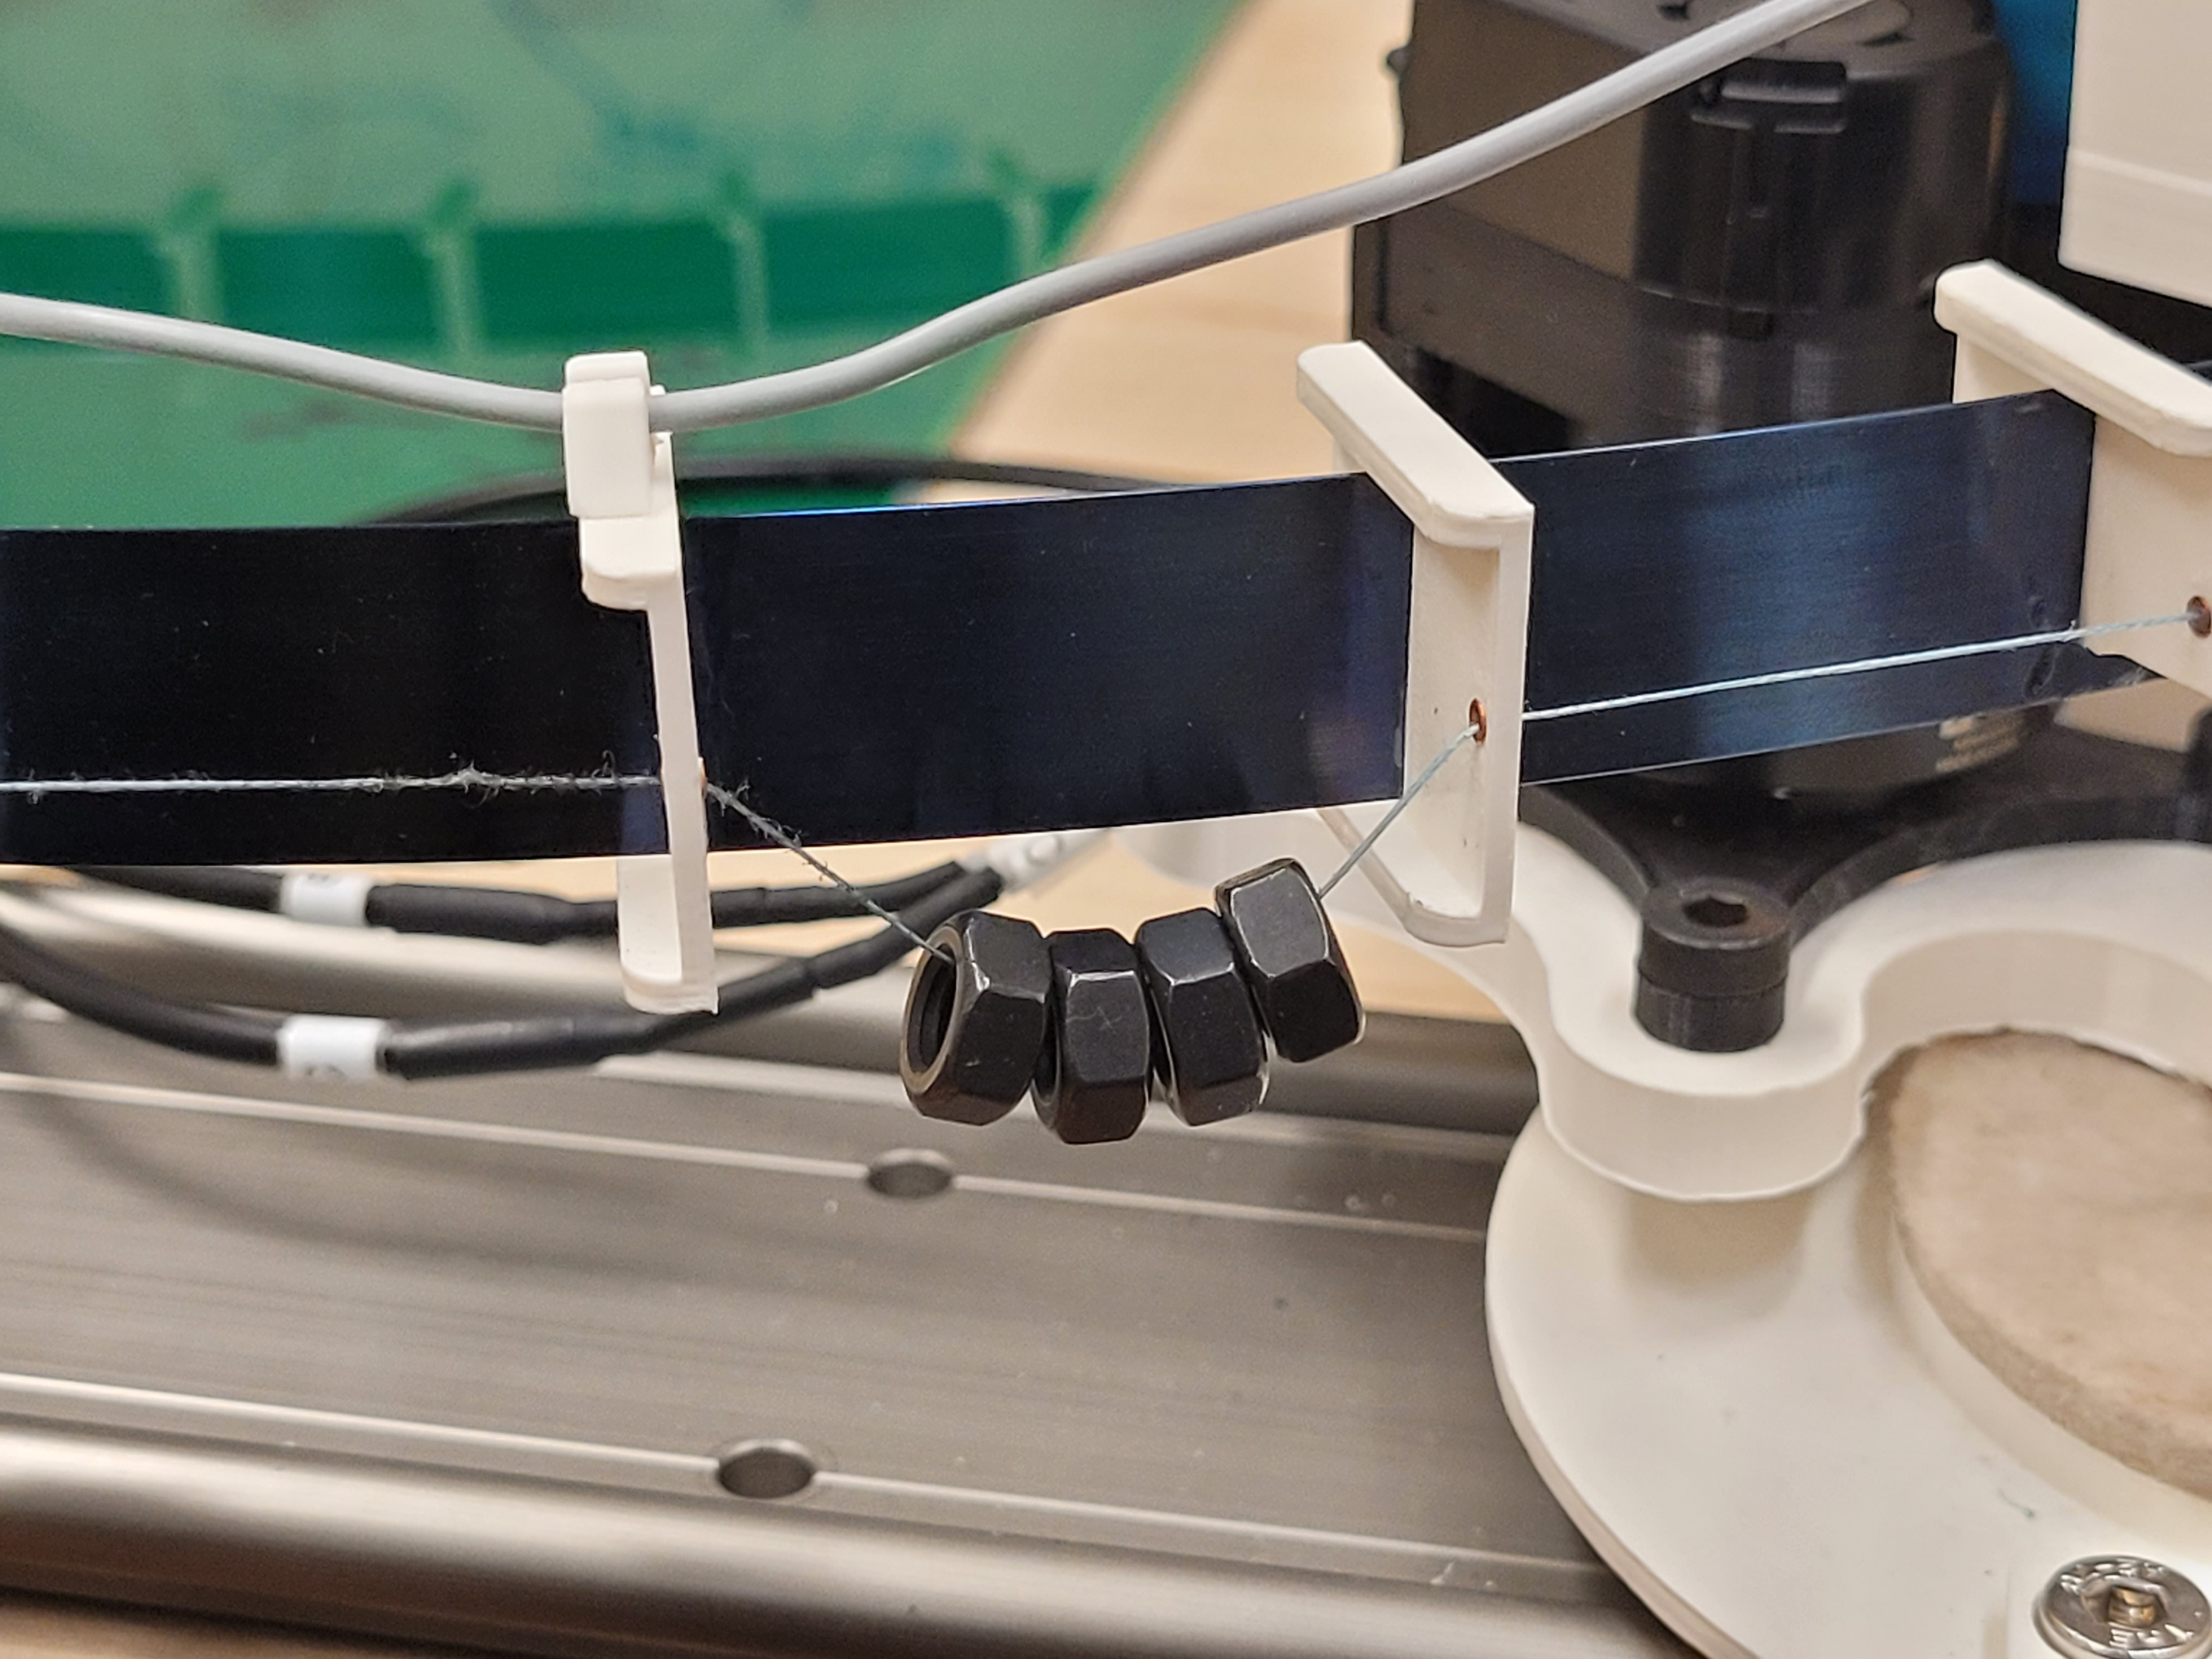
\includegraphics[width=0.5\textwidth]{images/tendon_slack.jpg}
    \caption{Four \SI{0.75}{"} nuts placed on a tendon to maintain tendon tension throughout operation}
    \label{fig:tendon_slack}
\end{figure}

% \begin{figure}[h]
%      \centering
%      \begin{subfigure}[b]{0.48\textwidth}
%          \centering
%          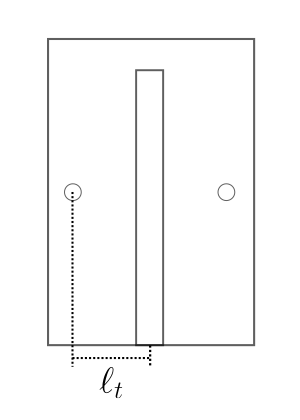
\includegraphics[width=0.625\textwidth]{images/beam_cross_section.png}
%          \caption{Cross section of the beam spacers. $\ell_t = \SI{11}{mm}$}
%          \label{fig:beam_cross_section}
%      \end{subfigure}
%      \hfill
%      \begin{subfigure}[b]{0.48\textwidth}
%          \centering
%          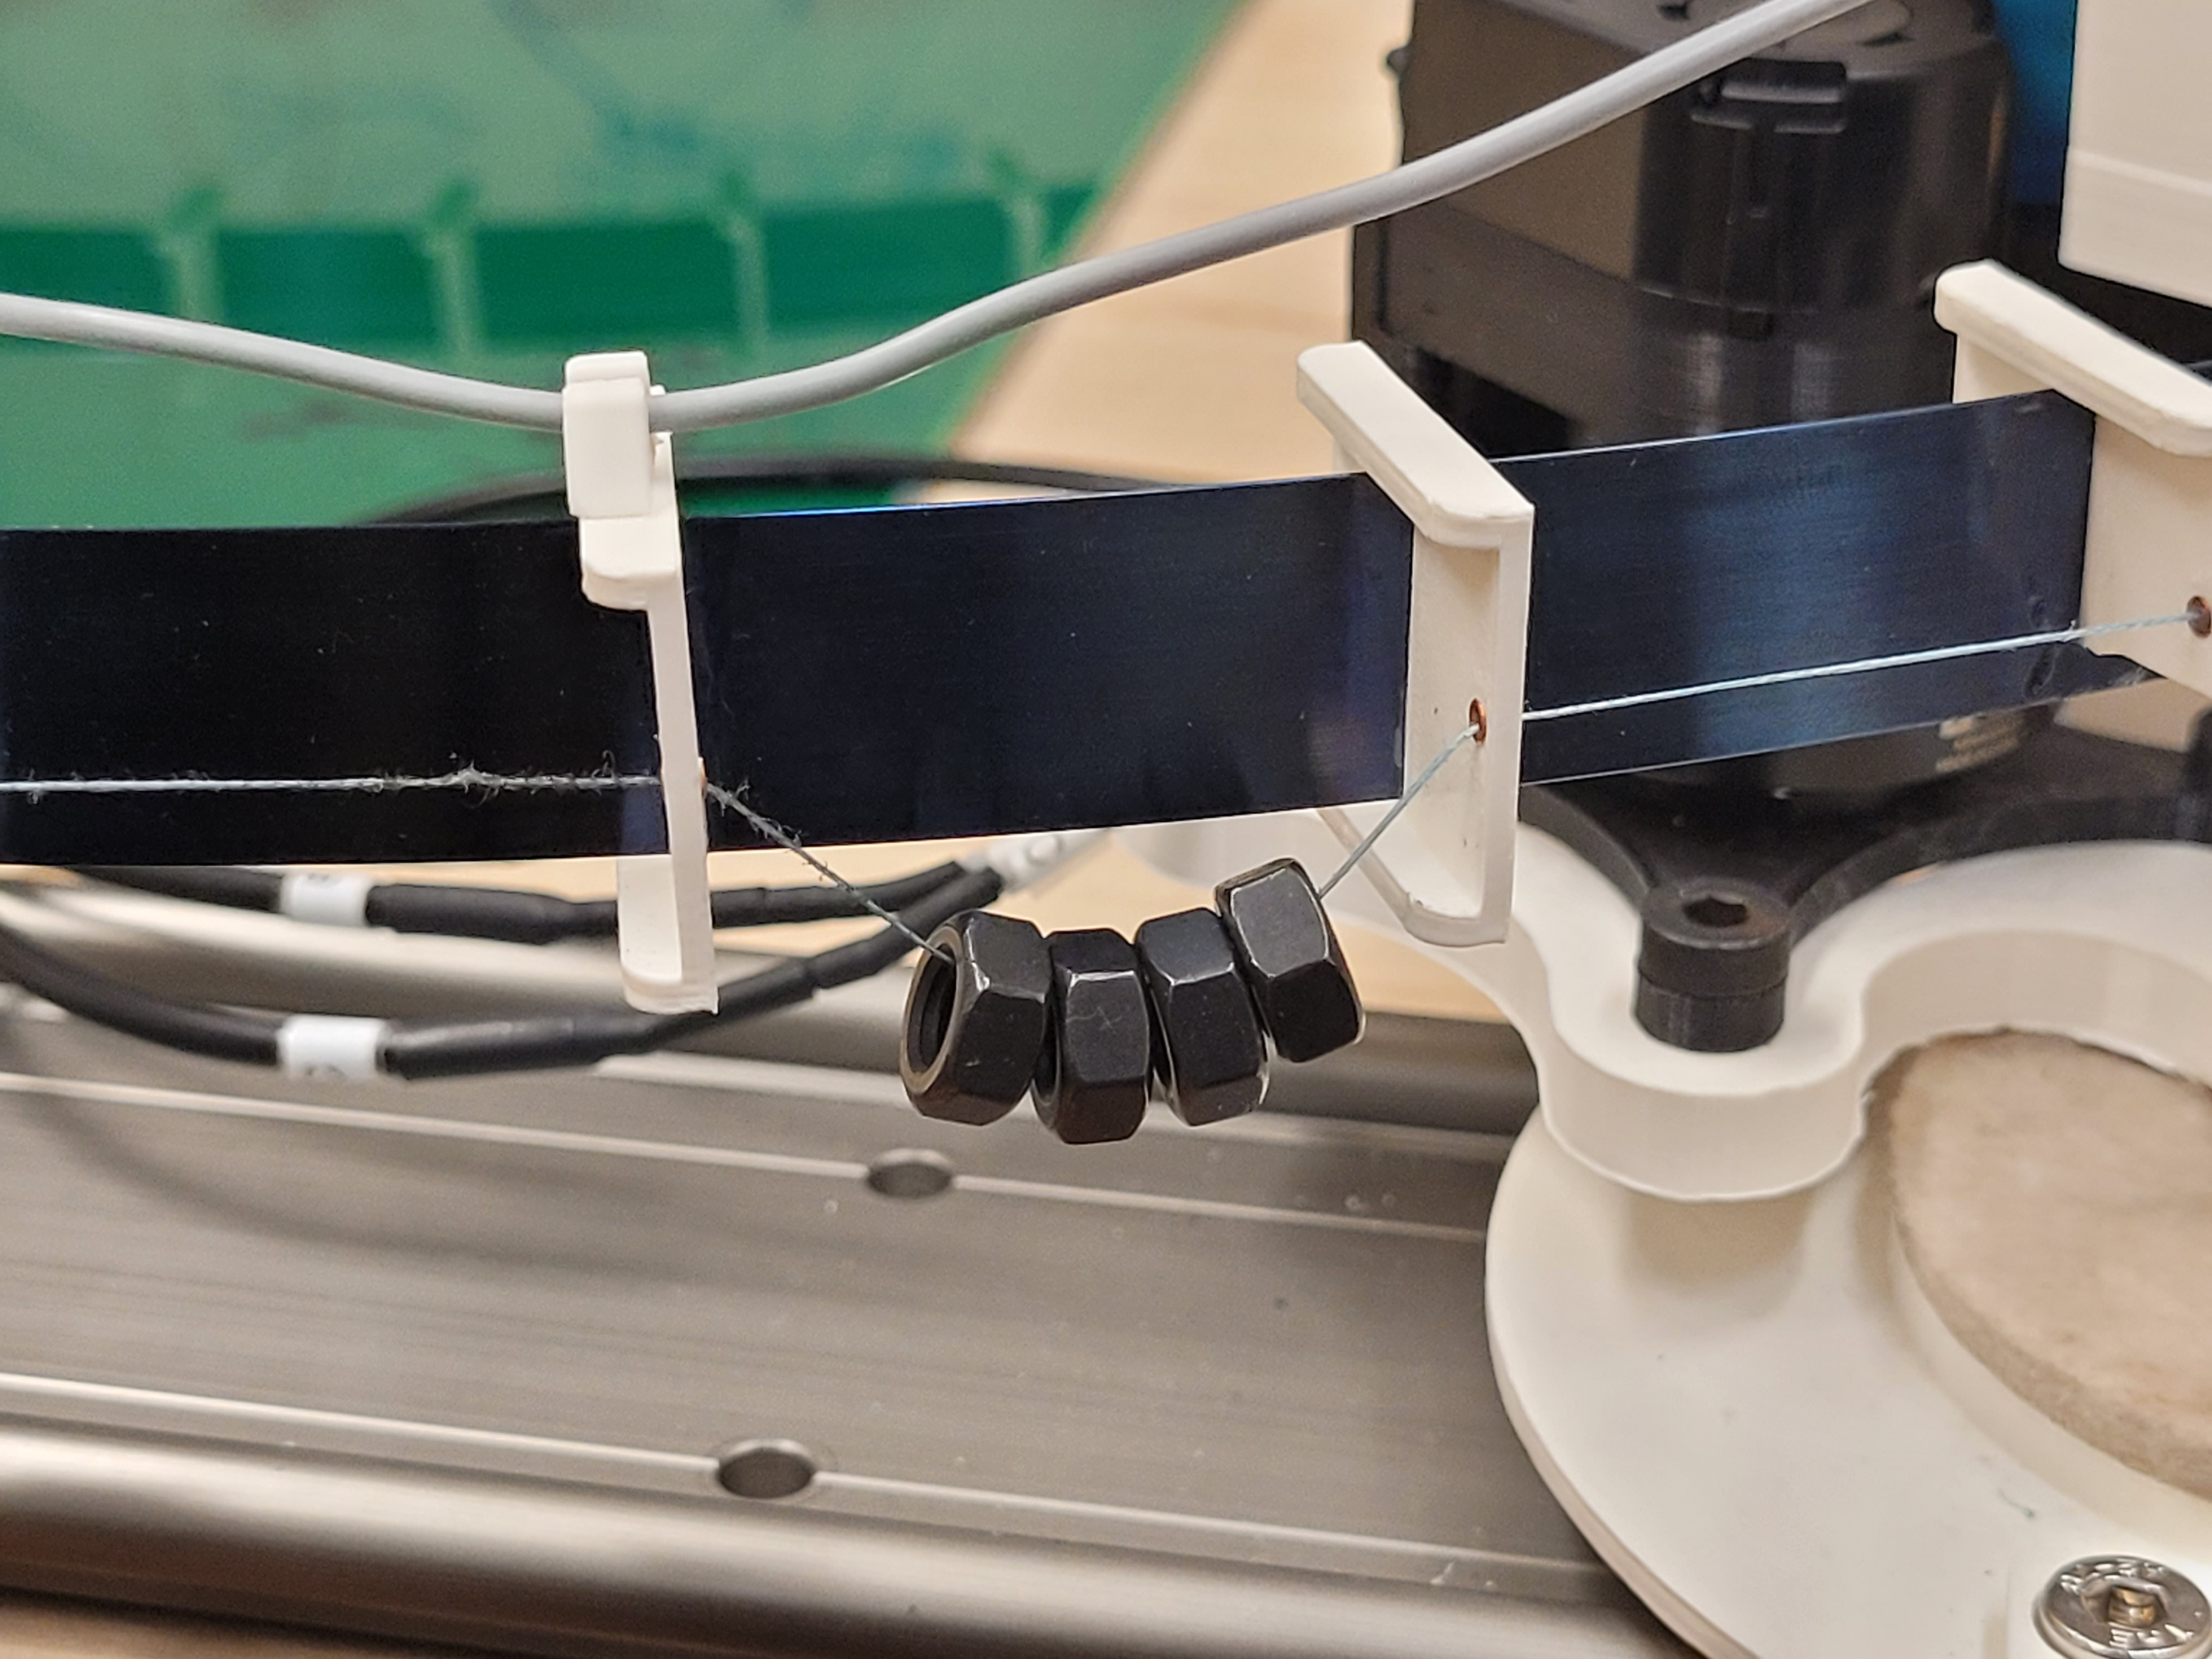
\includegraphics[width=\textwidth]{images/tendon_slack.jpg}
%          \caption{Four \SI{0.75}{"} nuts placed on a tendon to maintain tendon tension throughout operation}
%          \label{fig:tendon_slack}
%      \end{subfigure}
% \end{figure}

% Joints and End Effector  
\paragraph{The end effector} features a wide base to prevent the end effector from twisting off the plane. Revolute joints link the ends of each arm to the motor bases and the end effector, allowing both ends to rotate freely about the z-axis. The two arms share the same end effector. The bases for each arm are positioned \SI{60}{cm} apart.Each arm having its own independent degree of freedom grants the end effector in this configuration two degrees of freedom laying on the table plane. At this distance, the reachable workspace of the end effector covers a majority of the AURORA tracker workspace. During operation, a smaller end effector base does not provide enough area to balance the moments being applied by the two arms actuating the piece from different heights. Figure \ref{fig:ee_comparison} demonstrates this effect in action. Felt pads are attached to the bottom of the end effector to reduce friction between the end effector and table surface. 

\begin{figure}[h]
     \centering
     \begin{subfigure}[b]{0.48\textwidth}
         \centering
         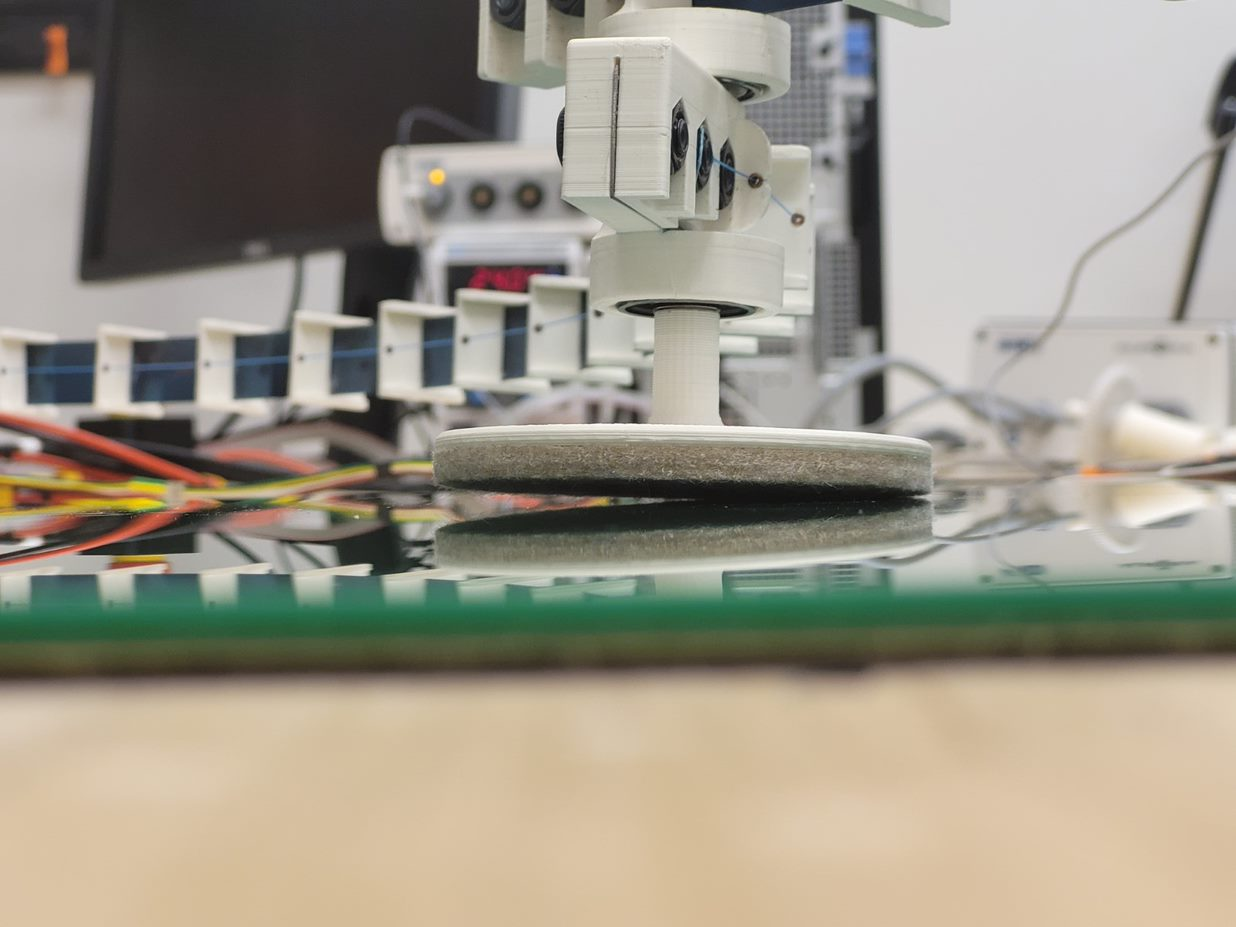
\includegraphics[width=\textwidth]{images/small_ee.jpeg}
         \caption{Smaller base causing the end effector to twist off the planar surface}
         \label{fig:small_ee}
     \end{subfigure}
     \hfill
     \begin{subfigure}[b]{0.48\textwidth}
         \centering
         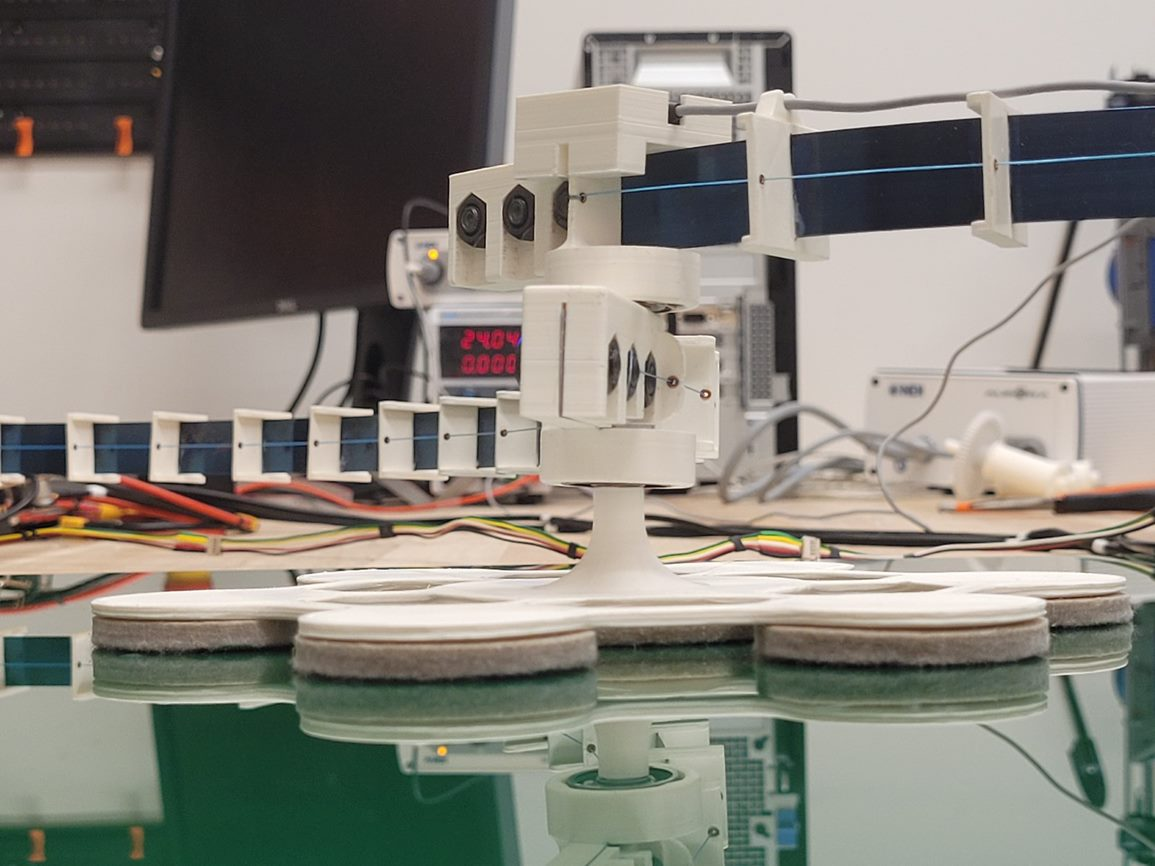
\includegraphics[width=\textwidth]{images/large_ee.jpeg}
         \caption{Larger base ensuring end effector remains on the plane}
         \label{fig:large_ee}
     \end{subfigure}
        \caption{Comparison of end effector sizes}
        \label{fig:ee_comparison}
\end{figure}

\paragraph{Gearboxes} are actuated directly by motors for each arm. The gear boxes are 3D printed but use purchase gears with a gear ratio of 16:1, enabling significantly higher applied torques than the motors are natively capable of. A 4:1 gear ratio is achieved by the motor unit. This results in a total gear ratio of 64:1 for the actuation unit. Each box contains two \SI{10}{mm} gears (2662N313, McMaster-Carr Supply Company, IL, USA) and three \SI{40}{mm} gears (2662N321, McMaster-Carr Supply Company, IL, USA) to achieve this rotation. The gearbox actuates a 3D printed spindle with a radius of \SI{11}{mm}. Two tendons are spooled around the spindle in opposite directions, so when it rotates, one tendon is extended while the other is contracted. Both tendons are firmly attached at the end effector side of each arm. This equal and opposite actuation of the tendons is what causes the arm to bend. 

% Workspace 
\paragraph{The workspace} additionally has an acrylic sheet used to reduce friction. Beneath the table surface, an AURORA electromagnetic tracking system (20-20 planar, Northern Digital Inc., ON, Canada) is positioned. The tracker is positioned to ensure maximal coverage of the robot's task space. The tracker is limited to an effective tracking area of \SI{50}{cm} x \SI{50}{cm} on the workspace plane. This unit tracks a wire coil which is fastened on the robot's end effector, directly above the revolute joint. This is where the end effector position is defined to be as a point in space. 

\subsubsection{Electronic Components}
Each arm is driven by a single Antigravity drone motor (MN4004 KV300, T-MOTOR, JX, P.R. China) which are both controlled by an off-the-shelf microprocessor (LAUNCHXL-F28069M, Texas Instruments, Dallas, USA) fitted with two booster cards (BOOSTXL-DRV8305EVM, Texas Instruments, Dallas, USA). The motors are part of an actuation unit shown in Figure \ref{fig:motor_unit} and contain a 4:1 gear ratio and an Avago optical encoder (AEDM 5810, Broadcom Inc., CA, USA) that is used to provide system feedback at a rate of \SI{1000}{hz} to the workstation. The actuation setup comes from the Open Continuum Robot project \cite{open_cr, Grimminger_2020}. A single micro-controller communicates with a workstation through the CAN bus protocol. The robot is powered using a \SI{240}{W} power supply operating at \SI{24}{V}. An emergency stop is installed within reach of the operator for safety. 

\begin{figure}[p]
    \centering
    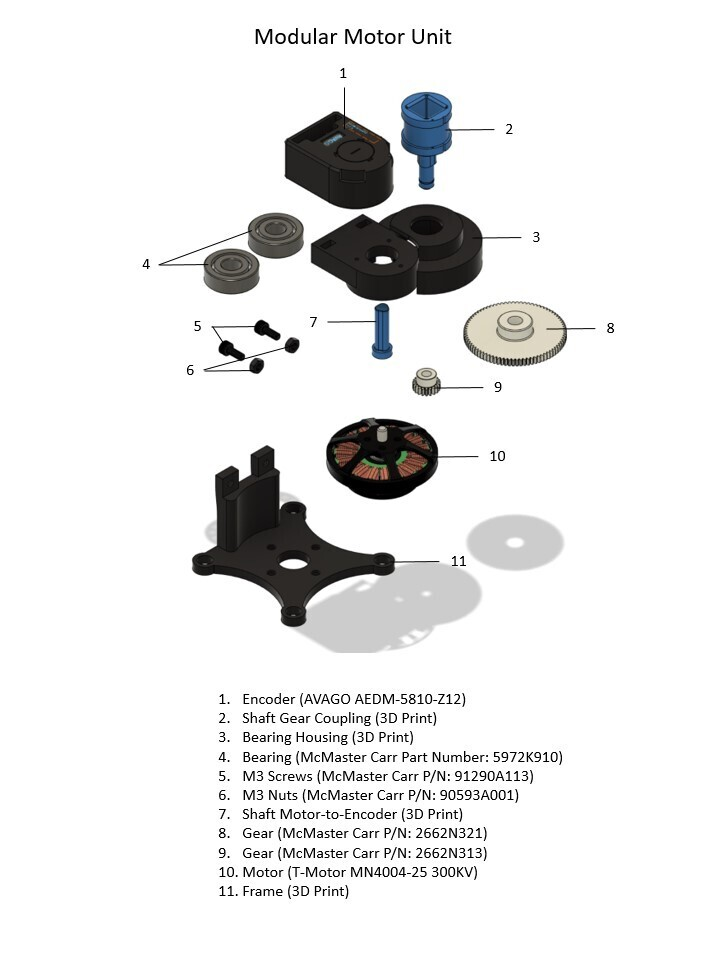
\includegraphics[width=\textwidth]{images/motor_unit.jpg}
    \caption{Complete schematic of the motor actuation unit, from \cite{motor_actuation_paper}}
    \label{fig:motor_unit}
\end{figure}

\paragraph{The workstation} used is a Dell OptiPlex 7090. It boasts an Intel Core i7-10700 CPU with 16GB of memory. It runs the RT-Preempt real time Linux kernel. The station communicates with the TI micro-controllers through a CAN-to-PCI Express interface card (IPEH-003027, PEAK system, Hessen, Germany). The station interfaces with the Aurora tracker through USB. Because the code for this thesis is written in Python, use of the real time kernel is not strictly required as Python does not support real time operations. For this project Python was deemed an appropriate language as it enables faster development times, and the shortcoming in terms of runtime is not seen to cause issues on the system. 

\subsubsection{Maximum Curvature Test}
Before the 16:1 gearbox was designed and installed, the actuation unit had a 4:1 gear ratio. An experiment was conducted to determine the arm length that enabled the largest range in the end effector position. Knowing the maximum and minimum distance that can be reached from an arm's base is required to set workspace bounds for the robot controller. The maximum distance is trivially given by the length of the arm. To find the minimum distance, a maximum curvature is applied by sending the highest current command a motor can support. The curvature that equates the bending forces to the maximum motor torque is taken as the maximum curvature. In this position, the distance between the end effector and arm base was measured. The results are displayed in Table \ref{tab:arm_length} and Figure \ref{fig:maximum_curve}. The arms were left at \SI{80}{cm} length as no notable gain in performance was observed at either test length. 

\begin{table}[h]
    \centering
    \caption{Arm distances during the maximum curvature test}
    \begin{tabular}{c|c|c}
        Extended Distance & Fully Contracted Distance & Contraction Distance \\
        \hline
        \SI{80}{cm} & \SI{59(1)}{cm} & \SI{21(1)}{cm} \\
        \SI{55}{cm} & \SI{33(1)}{cm} & \SI{22(1)}{cm} \\
    \end{tabular}
    \label{tab:arm_length}
\end{table}

This experiment showed the torque output of the motors resulted in a significantly smaller range of motion than what was initially expected. In response, a new gearbox was designed and manufactured to increase the maximum torque output of the robot. With the new gearbox, the robot is able to contract its arm completely with \SI{0}{cm} between the end effector and base. 

\begin{figure}[H]
     \centering
     \begin{subfigure}[b]{0.48\textwidth}
         \centering
         \includegraphics[width=\textwidth]{images/max_curve1.png}
         \caption{Without gearbox}
         \label{fig:maximum_curve1}
     \end{subfigure}
     \hfill
     \begin{subfigure}[b]{0.48\textwidth}
         \centering
         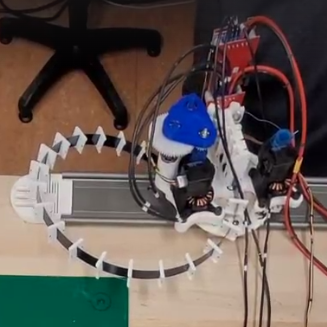
\includegraphics[width=\textwidth]{images/max_curve2.png}
         \caption{With gearbox}
         \label{fig:maximum_curve2}
     \end{subfigure}
        \caption{Maximum curvature tests}
        \label{fig:maximum_curve}
\end{figure}


\subsection{Baseline Controllers}
\label{sec:baseline_comparison}
Both the differential CC and PID baseline controllers were tested on three tasks: following a path, following a trajectory, and repeated the same motion. The results for each are presented in the following sections. The runtime of each controller is presented as well. 

\subsubsection{Path Tracking}
Both baseline controllers were asked to follow five test paths. Each path is discretized into ~50 way points. The controllers are required to measure an end effector position within \SI{2}{cm} of each way point before progressing to the next. The paths traced by each controller is shown in Figures \ref{fig:diff_cc_point_track} and \ref{fig:pid_point_track}. Table \ref{tab:baseline_test_point} highlights key metrics from each run including the total distance travelled by the robot and the time it took to complete each path. This test was repeated three times and the average results across all three trials are displayed. 

\begin{figure}[p]
    \centering
    \makebox[\textwidth][c]{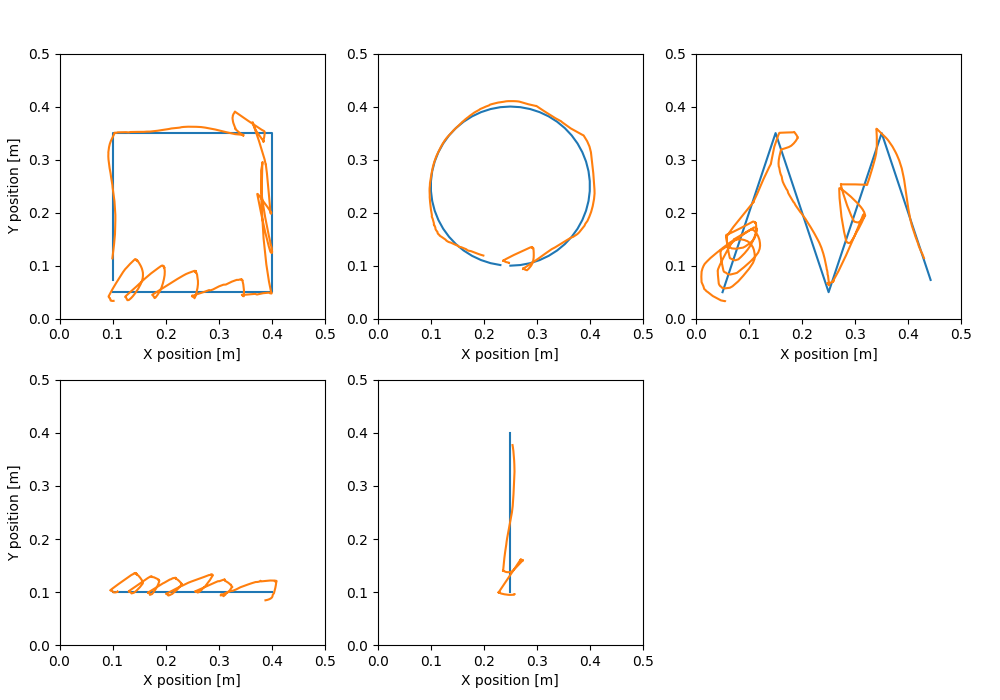
\includegraphics[width=0.95\textwidth]{images/diff_cc_point_tracking.png}}
    \caption{Differential CC controller point tracking path (orange) with reference path (blue) }
    \label{fig:diff_cc_point_track}
\end{figure}

\begin{figure}[p]
    \centering
    \makebox[\textwidth][c]{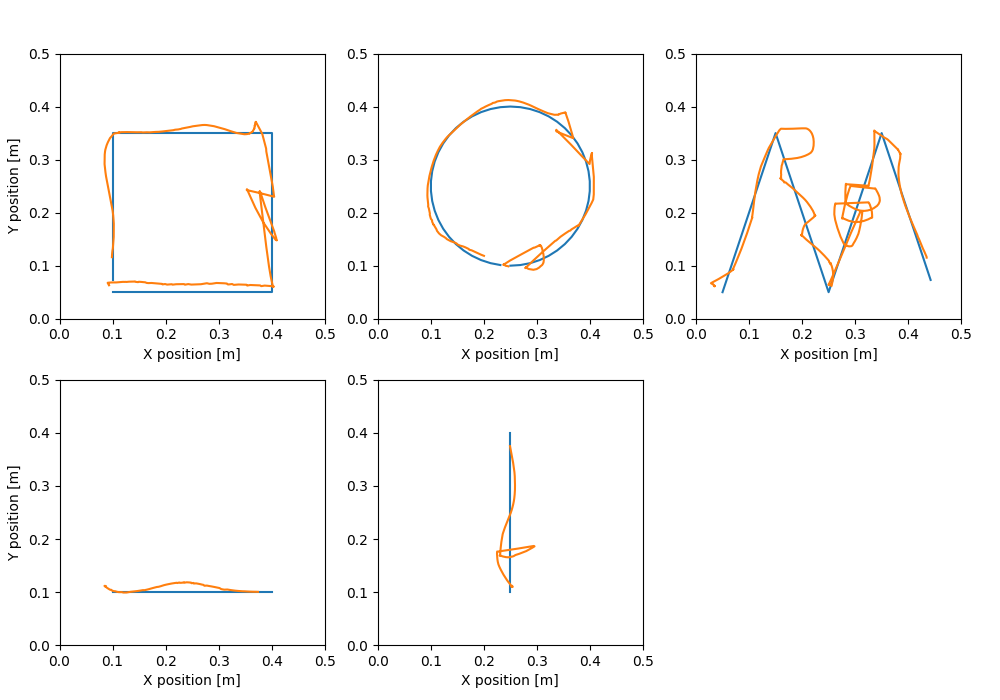
\includegraphics[width=0.95\textwidth]{images/pid_point_tracking.png}}
    \caption{PID controller point tracking path (orange) with reference path (blue)}
    \label{fig:pid_point_track}
\end{figure}

\begin{table}[h]
    \centering
    \caption{Baseline controller point tracking trial summary}
    \begin{tabular}{p{0.27\linewidth} | p{0.17\linewidth} | p{0.2\linewidth} | p{0.2\linewidth}}
        \textbf{Trial Shape} & \textbf{Run time [s]} & \textbf{Path Length [m]} & \textbf{Error}\\
        \hline
        \multicolumn{4}{c}{Reference Trajectory} \\
        \hline
        Square & N/A & 1.178 & N/A \\
        Circle & N/A & 0.923 & N/A \\
        Zig Zag & N/A & 1.241 & N/A \\
        Horizontal Line & N/A & 0.300 & N/A \\
        Vertical Line & N/A & 0.300 & N/A \\
        \hline
        \multicolumn{4}{c}{Differential CC Controller} \\
        \hline
        Square & 136.36 & 2.190 & 85.9\%\\
        Circle & 61.48 & 1.048 & 13.5\%\\
        Zig Zag & 152.21 & 2.551 & 105.6\%\\
        Horizontal Line & 105.48 & 0.817 & 172.3\%\\
        Vertical Line & 34.03 & 0.411& 37.0\%\\
        \hline
        \multicolumn{4}{c}{PID Controller} \\
        \hline
        Square & 74.92 & 1.454 & 23.4\%\\
        Circle & 87.58 & 1.197 & 29.7\%\\
        Zig Zag & 127.87 & 1.988& 60.2\%\\
        Horizontal Line & 19.01 & 0.302 & 0.6\%\\
        Vertical Line & 30.10 & 0.435 & 45\%\\
        \hline
    \end{tabular}   
    \label{tab:baseline_test_point}
\end{table}


\subsubsection{Trajectory Tracking}
Both baseline controllers were asked to execute five test trajectories in a set amount of time. Each trajectory is discretized into ~50 way points with \SI{0.2}{s} in between each. The robot is controlled to follow the way point as it progresses through each of the discretized points. The paths traced by each controller is shown in Figures \ref{fig:diff_cc_traj_track} and \ref{fig:pid_traj_track}. Table \ref{tab:baseline_test_traj} highlights key metrics from each run including the total distance travelled by the robot and the RMSE between the robot path and the test trajectory. 

\begin{figure}[p]
    \centering
    \makebox[\textwidth][c]{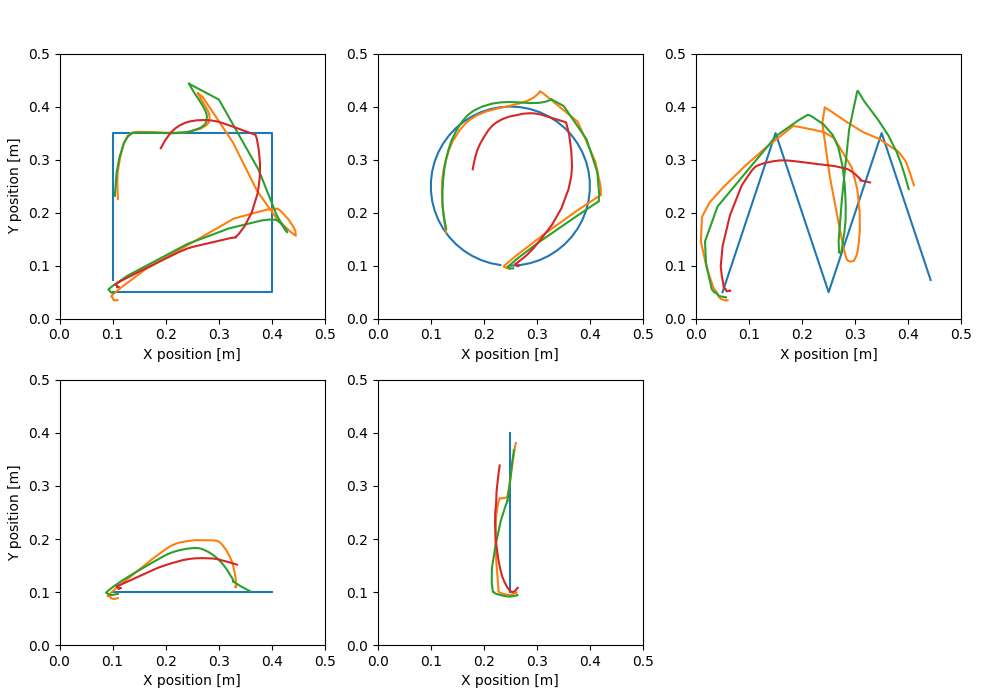
\includegraphics[width=0.95\textwidth]{images/diff_cc_traj_tracking.png}}
    \caption{Differential CC controller trajectory tracking paths (orange, green, red) with reference path (blue)}
    \label{fig:diff_cc_traj_track}
\end{figure}

\begin{figure}[p]
    \centering
    \makebox[\textwidth][c]{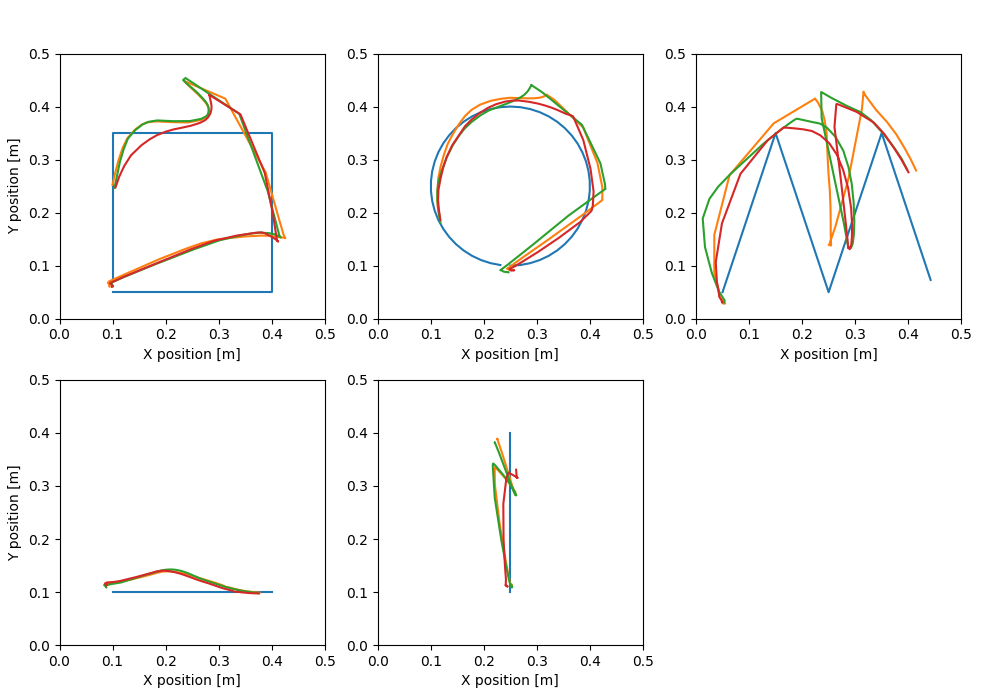
\includegraphics[width=0.95\textwidth]{images/pid_traj_tracking.png}}
    \caption{PID controller trajectory tracking paths (orange, green, red) with reference path (blue)}
    \label{fig:pid_traj_track}
\end{figure}

\begin{table}[h]
    \centering   
    \caption{Baseline controller trajectory tracking trial summary}
    \begin{tabular}{p{0.25\linewidth} | p{0.18\linewidth} | p{0.23\linewidth} | p{0.16\linewidth}}
        \textbf{Trial Shape} & \textbf{Run time [s]} & \textbf{Path Length [m]} & \textbf{RMSE [m]} \\
        \hline
        \multicolumn{4}{c}{Reference Trajectory} \\
        \hline
        Square & 10.80 & 1.178 & N/A\\
        Circle & 10.00 & 0.923 & N/A\\
        Zig Zag & 10.40 & 1.241 & N/A\\
        Horizontal Line & 10.20 & 0.300 & N/A\\
        Vertical Line & 10.20 & 0.300 & N/A\\
        \hline
        \multicolumn{4}{c}{Differential CC Controller} \\
        \hline
        Square & 12.25 & 0.959 & 0.144 \\
        Circle & 11.34 & 0.748 & 0.137 \\
        Zig Zag & 11.80 & 1.008 & 0.147 \\
        Horizontal Line & 11.57 & 0.324 & 0.072 \\
        Vertical Line & 11.57 & 0.305 & 0.055 \\
        \hline
        \multicolumn{4}{c}{PID Controller} \\
        \hline
        Square & 12.22 & 1.031 & 0.131 \\
        Circle & 11.31 & 0.833 & 0.124 \\
        Zig Zag & 11.77 & 11.213 & 0.150 \\
        Horizontal Line & 11.54 & 0.306 & 0.043 \\
        Vertical Line & 11.54 & 0.360 & 0.054 \\
        \hline
    \end{tabular}
    \label{tab:baseline_test_traj}
\end{table}


\subsubsection{Task Repetition}
Controllers were tested on their ability to repeat the same task consistently. The trial was run from home position to the point (\SI{0.15}{m}, \SI{0.2}{m}). It was repeated 10 times for each controller. The paths taken by each controller are shown in Figure \ref{fig:repetition_trial}. The maximal Fréchet distance \cite{frechet_distance} is calculated between each of the 10 trials for both controllers as a metric of controller consistency. The differential CC controller has a maximal Fréchet distance of \SI{0.102}{m} while the PID controller has a maximal Fréchet distance of \SI{0.027}{m}, indicating a much tighter distribution. This result is confirmed visually in Figure \ref{fig:repetition_trial}. 

\begin{figure}[h]
     \centering
     \begin{subfigure}[b]{0.48\textwidth}
         \centering
         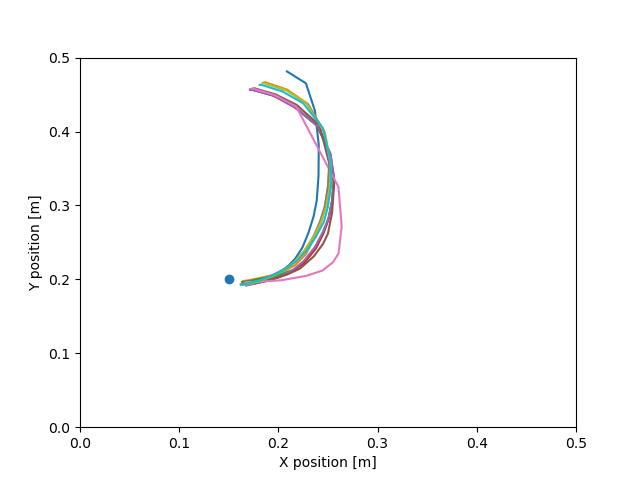
\includegraphics[width=\textwidth]{images/diff_cc_repetition.png}
         \caption{Differential CC controller task repetition}
         \label{fig:diff_cc_repetition}
     \end{subfigure}
     \hfill
     \begin{subfigure}[b]{0.48\textwidth}
         \centering
         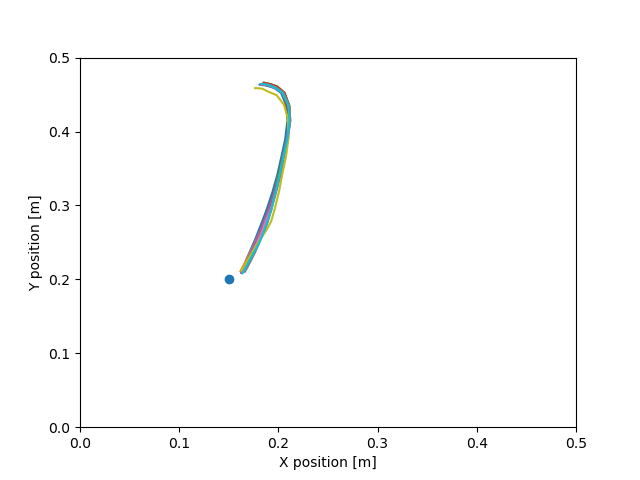
\includegraphics[width=\textwidth]{images/pid_repetition.png}
         \caption{PID controller task repetition}
         \label{fig:pid_repetition}
     \end{subfigure}
        \caption{Baseline controller repeated motion trial paths. The target point is shown in blue.}
        \label{fig:repetition_trial}
\end{figure}


\subsubsection{Timing Analysis}
The runtime of four different necessary controller functions was studied for both baseline controllers and the best performing learned controller. This includes the controller constructor method, the command retrieval, the end point update, and the goal point update. Table \ref{tab:runtimes} displays the results. A "per iteration" result is returned as well, which is a sum of the three functions that are required to run at each control loop. 

\begin{table}[h]
    \centering   
    \caption{Controller run times}
    \begin{tabular}{p{0.4\linewidth} | p{0.2\linewidth} }
        \textbf{Function} & \textbf{Run time [$\mu$s]} \\
        \hline
        \multicolumn{2}{c}{Differential CC Controller} \\
        \hline
        Current command retrieval & 0.1 \\
        End point update & 364.2 \\
        Goal point update & 0.2 \\
        \textbf{Total per iteration} & \textbf{364.5} \\
        Controller object construction & 11.4 \\
        \hline
        \multicolumn{2}{c}{PID Controller} \\
        \hline
        Current command retrieval & 0.1 \\
        End point update & 24.5 \\
        Goal point update & 0.8 \\
        \textbf{Total per iteration} & \textbf{25.4} \\
        Controller object construction & 211.0 \\
        \hline
        \multicolumn{2}{c}{Learning-Based Controller} \\
        \hline
        Current command retrieval & 0.2 \\
        End point update & 356.3 \\
        Goal point update & 0.2 \\
        \textbf{Total per iteration} & \textbf{356.7} \\
        Controller object construction & 1,184.3 \\
        \hline
    \end{tabular}
    \label{tab:runtimes}
\end{table}


\subsection{Learning Pipeline}
\subsubsection{Learning Tasks}
Several behaviours were witnessed throughout data collection that pose interesting learning challenges for users of this dataset. By only providing the end effector position, no information is explicitly provided about the curvature of the robot. Cases arise where the robot can take on different shapes given the same end effector position by making use of the external forces applied on the end effector. An example of this is shown in Figure \ref{fig:multiple_solutions}. The two arms shown would have different dynamic behaviour during operation and so it may be valuable to have systems that have state representations larger than just an end effector position. This idea is what motivated the use of a larger LSTM layer in the learning-based controller state estimation sub-model. 

\begin{figure}[h]
    \centering
    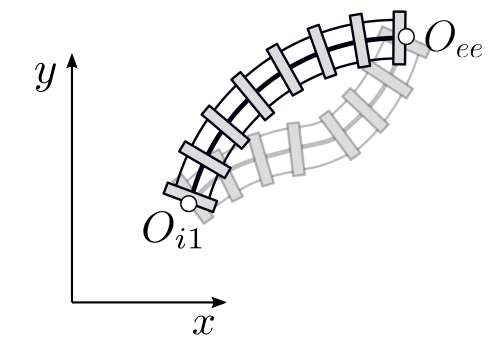
\includegraphics[width=0.5\textwidth]{images/multiple_solutions.png}
    \caption{Example of two robot configurations with equal tendon displacements}
    \label{fig:multiple_solutions}
\end{figure}

Another behaviour relating to the tendon slack issue discussed in Section \ref{sec:prototype_limitations_discussion} is exacerbated in the dataset because of the beam spring effect. When the robot's arm is being contracted, a restoring force acts on the end effector. If this restorative force is large enough, when the robot switches between contracting and extension the end effector will jump slightly to achieve tension in the tendon on the other side of the arm. For this to happen, the restorative force must be great enough to overcome static friction between the end effector and the table. This behaviour can be very sudden and is what results in the significantly higher maximum velocity during robot extension. When the restoring force is not great enough to overcome static friction, a period of time will pass where the motor is actuated with no end effector motion. There are only certain states that allow for this stationary behaviour to occur and it is not clear how to explicitly find them, they are not solely related to end effector position. Figure \ref{fig:equillibrium_position} shows one such equilibrium state. 

\begin{figure}[h]
    \centering
    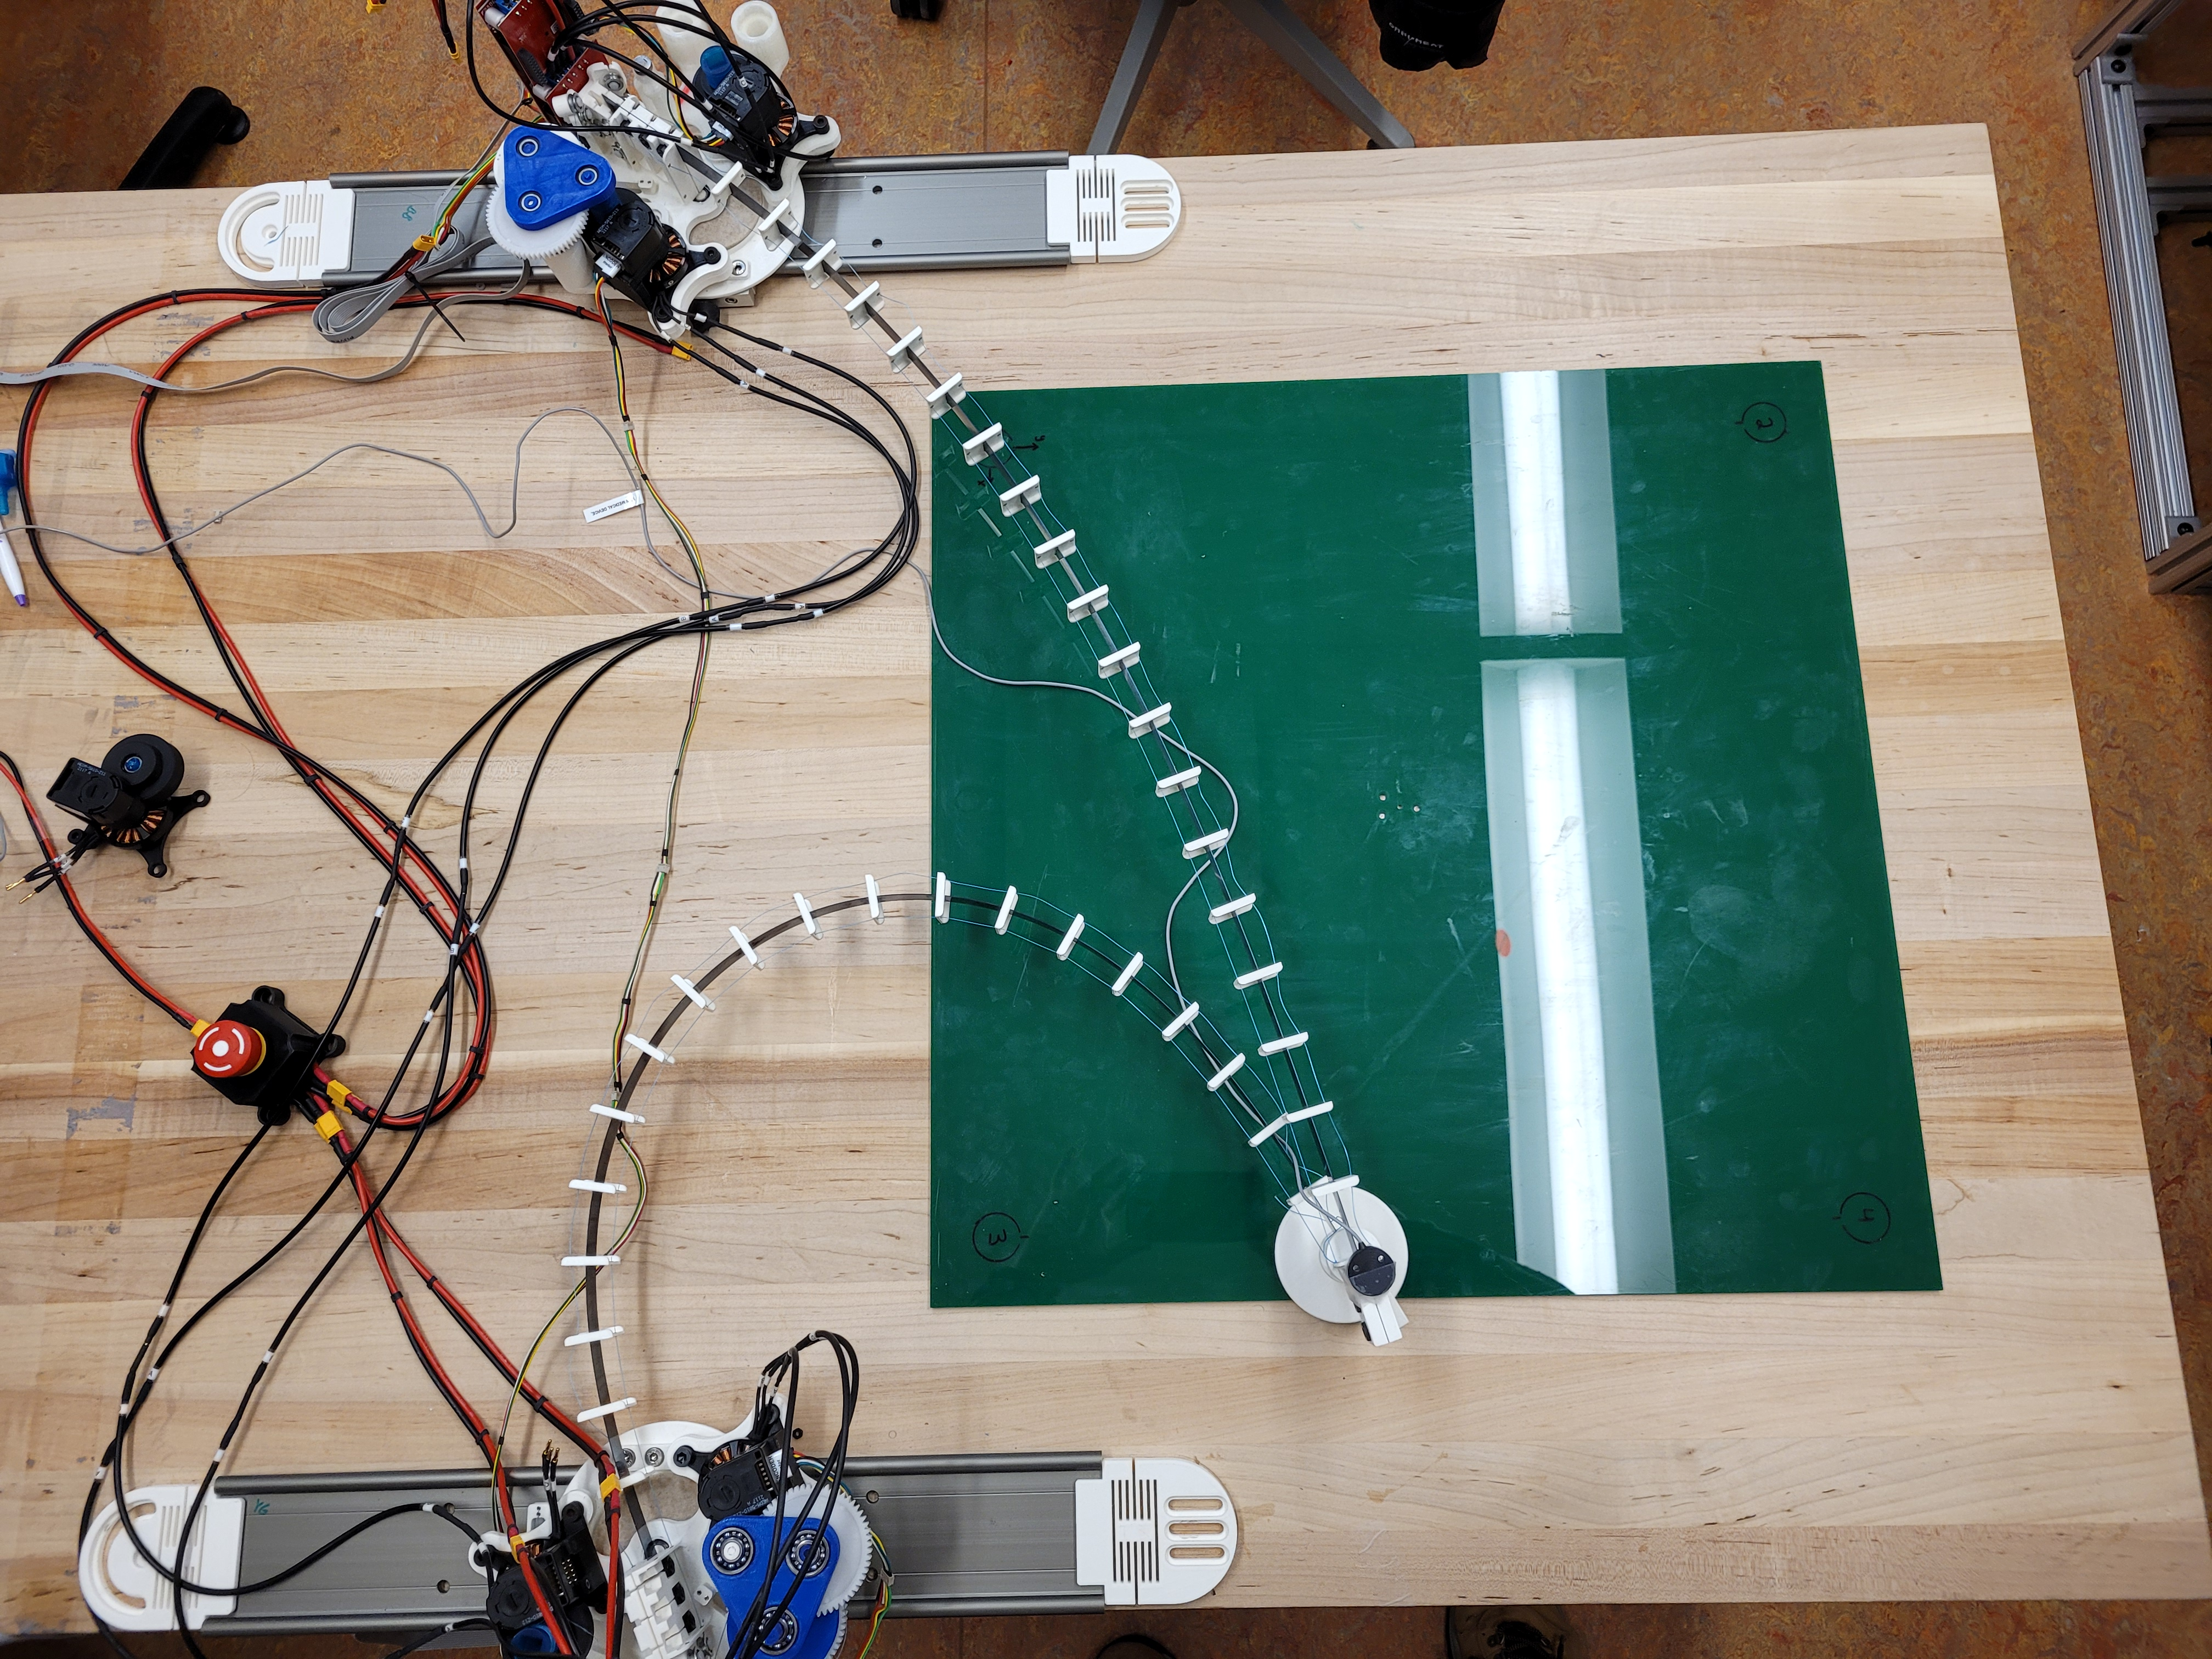
\includegraphics[width=0.5\textwidth]{images/equillibrium_location.jpg}
    \caption{Example of an equilibrium position where the robot will remain stationary despite motor actuation}
    \label{fig:equillibrium_position}
\end{figure}

\subsubsection{Expected Impact}
Learning-based approaches have the potential to model arbitrarily complex dynamic systems. Using this dataset, the expectation is that learning-based controllers will greatly improve upon the baseline accuracy. This is especially true when the model is moving fast or bending far, where the baseline model assumptions are less accurate. These models will be able to more accurately estimate the system kinematics and dynamics, enabling real-time tracking in task space for this robot. 

While there does not exist a direct comparison in the literature to the proposed parallel planar system, several references suggest that accuracy results in the range of 0.5-2\% of the robot's length could be expected with further controller development \cite{grassmann2022a, 7112506, 10.3389/frobt.2021.730330}. As this is the first step towards learning-based control being proposed for a PCR, accuracy comparable with current state-of-the-art for other CRs is only useful to provide a ballpark of what is possible. 


\subsection{Open Continuum Robotics}
With the rise in popularity of continuum robots, the Open Continuum Robotics project was created to reduce barriers to entry into the field \cite{open_cr}. The work of this thesis will be open sourced and aims to contribute to the Open CR project. Throughout the design process, keeping the robot easy to reproduce and repair influenced the design to enable third parties to recreate the setup. All parts are either off-the-shelf or 3D printed, with all firmware being open-source. This work helps bridge the gap between CRs and machine learning while removing barriers to access for other researchers to explore this problem. 

